\documentclass[11pt,a4paper]{article}

\usepackage[T1]{fontenc}
\usepackage[utf8]{inputenc}
\usepackage{lmodern}
\usepackage[margin=22mm]{geometry}
\usepackage{graphicx}
\usepackage{booktabs}
\usepackage{array}
\usepackage{amsmath}
\usepackage{amssymb}
\usepackage{siunitx}
\usepackage{xcolor}
\usepackage{hyperref}
\usepackage{caption}
\usepackage{subcaption}

\sisetup{detect-all=true, round-mode=places, round-precision=3}
\graphicspath{{figures/}}

\title{Results III: Pre-registered Transferability to Hydronic-Family BOPTEST Testcases}
\author{Standalone Overleaf section generated from the HVAC\_DRL\_MORL Block 3 artifacts}
\date{June 2026}

\begin{document}
\maketitle

\section{Block 3 objective and claim boundary}

Blocks 1 and 2 established the source-case recipe on BOPTEST \texttt{bestest\_air}: a v3 rollout surrogate supplies smooth control-oriented dynamics, a calibrated v3.5 RC--NeuralODE supplies a frozen physical disagreement censor, and the thermostatic PPO policy trained on the resulting hybrid backend is the strongest verified controller on the targeted windows. Block 3 asks a narrower and more falsifiable question: does this fixed source-case recipe transfer to related BOPTEST hydronic-family testcases?

The claim boundary is deliberately limited. Block 3 does not claim universal building generalization, cross-climate generalization, or transfer to arbitrary HVAC topologies. It evaluates transfer to three pre-selected single-zone hydronic-family cases under documented actuator adapters and pre-registered recalibration regimes. Controller fine-tuning on the target testcase is explicitly excluded. This exclusion is methodologically important because it separates controller transfer from surrogate recalibration transfer.

Figure~\ref{fig:protocol} summarizes the protocol. The frozen Block 2 controller is routed through a testcase-specific actuator adapter and evaluated against the testcase's built-in PI baseline. In parallel, the v3.5 inverse-calibration pipeline is re-run under increasing recalibration depth: none, partial, and full. The resulting evidence is therefore component-level: controller-side transfer and surrogate-side transfer are reported separately.

\begin{figure}[t]
  \centering
  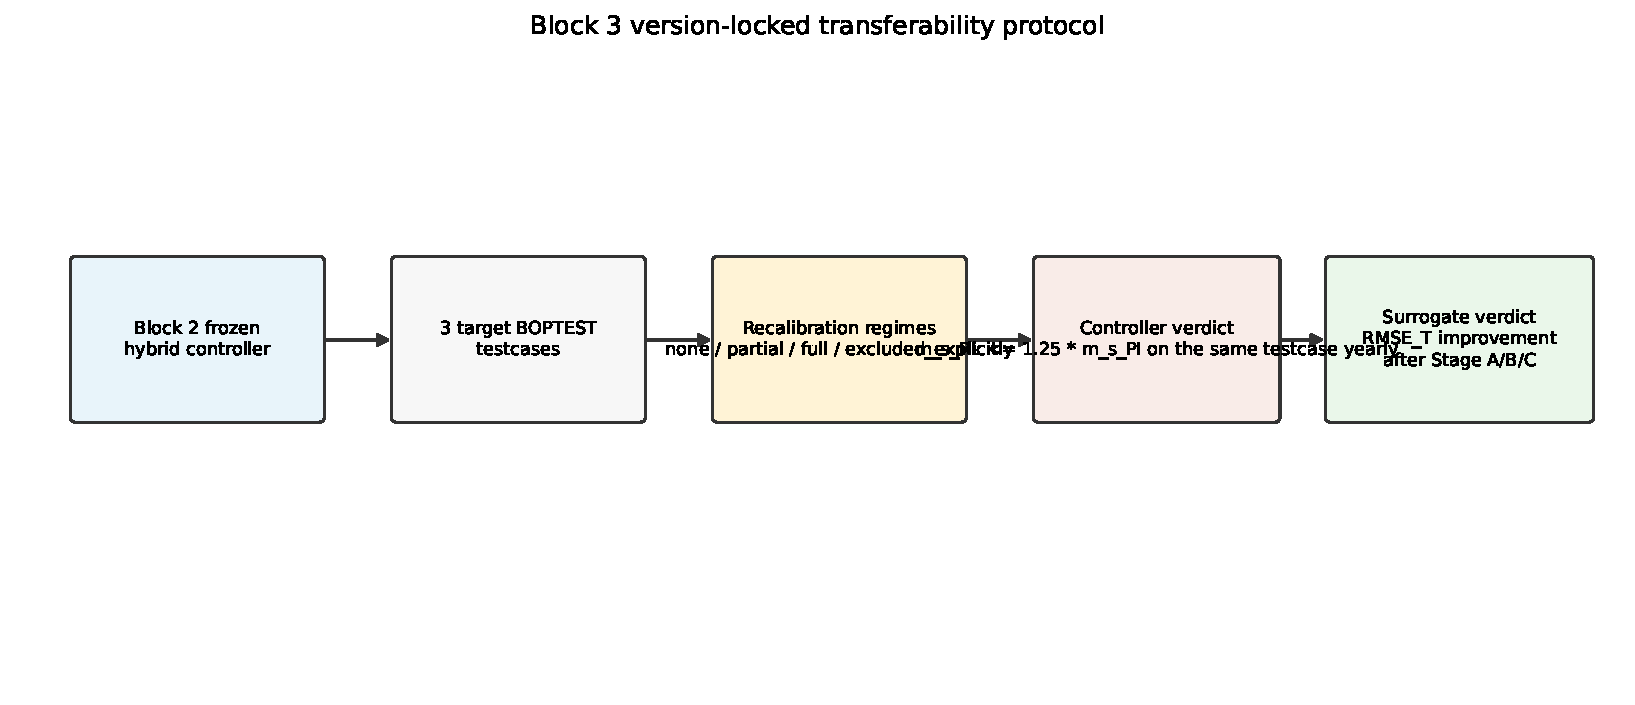
\includegraphics[width=0.94\linewidth]{final17_fig11_block3_transferability_protocol.pdf}
  \caption{Block 3 pre-registered transferability protocol. Controller-side transfer is tested against a testcase-specific PI threshold, while surrogate-side transfer is tested by full Stage A/B/C recalibration on target telemetry.}
  \label{fig:protocol}
\end{figure}

\section{Pre-registration and audit anchors}

Block 3 is pre-registered through \texttt{configs/block3\_testcase\_manifest.yaml}. The initial manifest commit (\texttt{1861e48}) was made before any non-\texttt{bestest\_air} BOPTEST run. The subsequent audit commits record the manifest SHA, actuator-adapter specifications, stretch-testcase predictions, close SHA, and interpretation. The relevant audit anchors are:
\begin{itemize}
  \item \texttt{1861e48}: Block 3 pre-registration manifest.
  \item \texttt{2f9d596}: record pre-registration commit SHA.
  \item \texttt{eb7091e}: hydronic heat-pump actuator adapter.
  \item \texttt{46fbaa9}: \texttt{bestest\_hydronic} direct supply adapter.
  \item \texttt{645626e}: commercial hydronic adapter and stretch-testcase predictions.
  \item \texttt{7ada793}: record close commit SHA.
  \item \texttt{cb7025f}: component-level transferability interpretation and threshold-pass caveat.
\end{itemize}
The registration block is preserved as an audit artifact; results are appended rather than retroactively editing the hypothesis definitions.

\section{Testcases, actuator adapters, and regimes}

The three target testcases span an increasing difficulty ladder relative to \texttt{bestest\_air}. All are single-zone or single-zone-like, heating-capable, and structurally non-identical to the source case.

\begin{table}[t]
\centering
\caption{Pre-registered target testcases and actuator adapters.}
\label{tab:testcases}
\small
\begin{tabular}{llll}
\toprule
Role & Testcase & Structural difference & Adapter \\
\midrule
Primary & \texttt{bestest\_hydronic\_heat\_pump} & hydronic loop + heat pump & \texttt{hydronic\_t\_supply\_to\_setpoint\_v1} \\
Secondary & \texttt{bestest\_hydronic} & boiler/radiator hydronic distribution & \texttt{hydronic\_direct\_supply\_setpoint\_adapter\_v1} \\
Stretch & \texttt{singlezone\_commercial\_hydronic} & larger commercial zone + hydronic valve & \texttt{commercial\_hydronic\_supply\_valve\_adapter\_v1} \\
\bottomrule
\end{tabular}
\end{table}

\begin{figure}[t]
  \centering
  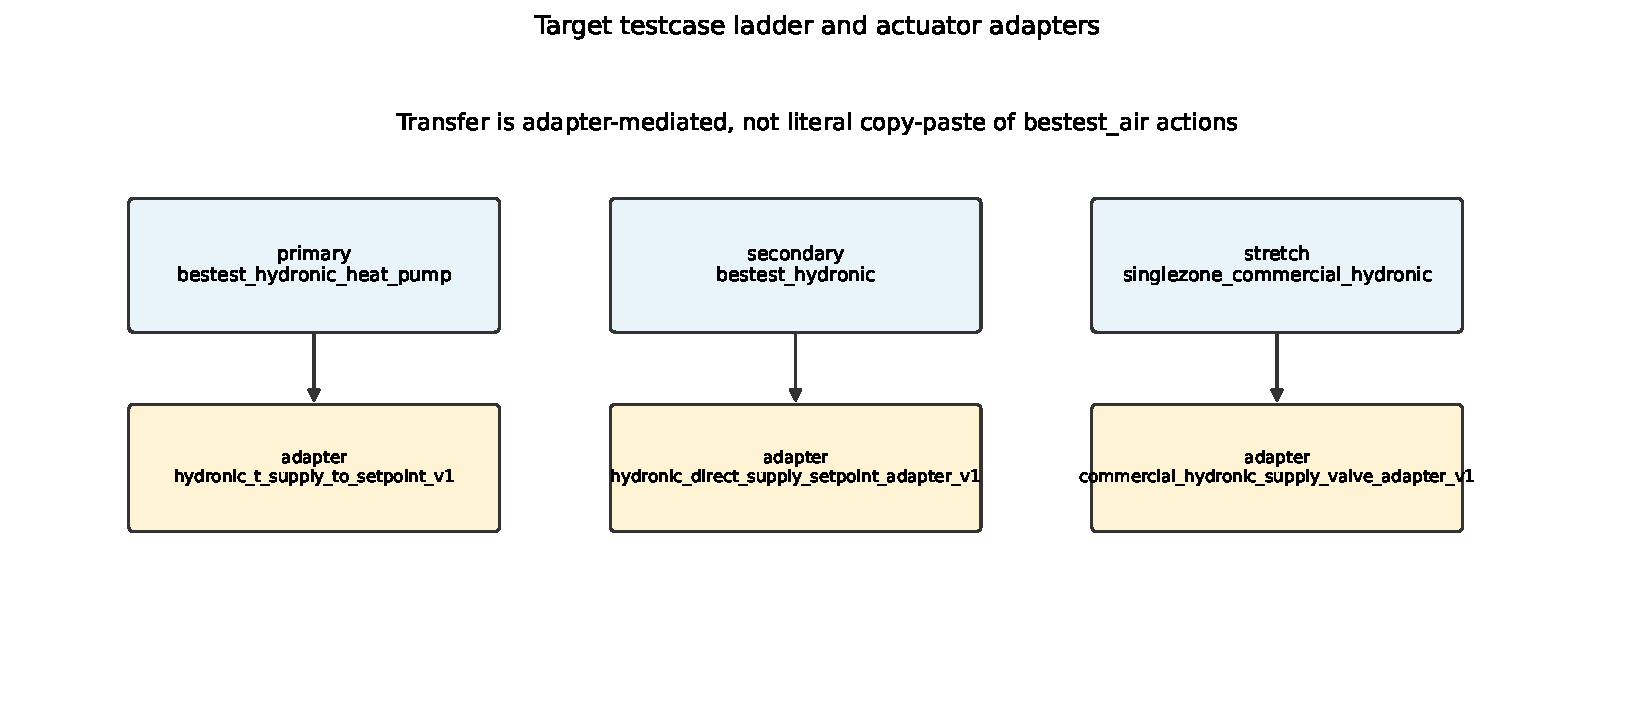
\includegraphics[width=0.92\linewidth]{final17_fig12_target_testcase_ladder_adapters.pdf}
  \caption{Target-testcase ladder and actuator-interface adapters. The transfer experiment is adapter-mediated, not a literal copy-paste of the \texttt{bestest\_air} supply-temperature actuator.}
  \label{fig:adapters}
\end{figure}

The adapter layer maps the source controller's normalized supply-temperature-like action to the target testcase's actuator interface:
\begin{equation}
  u^{\mathrm{target}}_t =
  \mathcal{A}_{k}
  \left(
  T^{\mathrm{sup}}_t,\,
  y_t
  \right),
  \qquad
  T^{\mathrm{sup}}_t =
  18 + \frac{a_t+1}{2}(35-18),
  \label{eq:adapter}
\end{equation}
where $\mathcal{A}_{k}$ is the pre-registered adapter for testcase $k$, $a_t\in[-1,1]$ is the frozen policy output, and $y_t$ denotes available BOPTEST measurements used by rule-based adapter logic. Smoke tests verify that low and high override conditions produce directionally valid heating responses before any yearly controller run.

The recalibration regimes isolate how much of the surrogate component is allowed to adapt:
\begin{table}[t]
\centering
\caption{Pre-registered recalibration regimes. The controller is frozen in every regime.}
\label{tab:regimes}
\small
\begin{tabular}{lll}
\toprule
Regime & Surrogate action & Controller action \\
\midrule
none & frozen \texttt{bestest\_air} surrogate recipe & frozen Block 2 hybrid controller \\
partial & Stage C residual-head recalibration only & frozen Block 2 hybrid controller \\
full & Stage A + Stage B + Stage C on target telemetry & frozen Block 2 hybrid controller \\
\bottomrule
\end{tabular}
\end{table}

\section{Engineering metrics and pass/fail rules}

The controller-side pass threshold is normalized by each testcase's built-in PI baseline:
\begin{equation}
  \tau_k = 1.25\,m_{s,\mathrm{PI},k},
  \qquad
  q_k =
  \frac{m_{s,\mathrm{RL},k}}{\tau_k}.
  \label{eq:threshold_ratio}
\end{equation}
The pre-registered threshold verdict is
\begin{equation}
  \mathrm{PASS}_{k}^{\mathrm{controller}}
  =
  \mathbb{I}
  \left[
  q_k \le 1
  \right].
  \label{eq:controller_pass}
\end{equation}
This is a safety/composite-metric threshold, not a complete deployment verdict. Energy is therefore reported separately:
\begin{equation}
  \Delta E_k(\%) =
  100\,
  \frac{E_{\mathrm{RL},k}-E_{\mathrm{PI},k}}
       {E_{\mathrm{PI},k}}.
  \label{eq:energy_delta}
\end{equation}
The commercial testcase illustrates why this two-axis reporting is needed: it passes the $m_s$ threshold but consumes substantially more energy than PI.

Surrogate-side transfer is measured by the relative improvement of target-testcase rollout RMSE after full Stage A/B/C recalibration:
\begin{equation}
  G^{\mathrm{RMSE}}_k(\%) =
  100\,
  \frac{
  \mathrm{RMSE}^{\mathrm{raw}}_{T,k}
  -
  \mathrm{RMSE}^{\mathrm{full}}_{T,k}
  }
  {\mathrm{RMSE}^{\mathrm{raw}}_{T,k}}.
  \label{eq:rmse_gain}
\end{equation}
The physical transfer diagnostic is the target re-identified capacitance ratio:
\begin{equation}
  \rho_{C,k} =
  \frac{C_{\mathrm{zon},k}}{C_{\mathrm{zon},\mathrm{bestest\_air}}},
  \qquad
  C_{\mathrm{zon},\mathrm{bestest\_air}} = 4.413\times10^5\,\mathrm{J/K}.
  \label{eq:czon_ratio}
\end{equation}

\section{Headline transfer matrix}

Table~\ref{tab:transfer_matrix} is the compact evidence summary. It contains two different stories. The surrogate component transfers strongly: full Stage A/B/C improves RMSE by $60.2$--$87.8\%$ on all three target testcases. The frozen controller does not transfer uniformly: the two residential hydronic cases fail the pre-registered $1.25\times$ PI threshold, while the commercial stretch case passes the threshold but pays a $+35.3\%$ energy penalty.

\begin{table}[t]
\centering
\caption{Block 3 transfer matrix. Threshold is $1.25\times m_{s,\mathrm{PI}}$ per testcase.}
\label{tab:transfer_matrix}
\scriptsize
\begin{tabular}{lrrrrrrrr}
\toprule
Testcase & $m_s^{RL}$ & $m_s^{PI}$ & Threshold & Ctrl. verdict & $\Delta E$ \% & Raw RMSE & Full RMSE & $C_{\mathrm{zon}}$ ratio \\
\midrule
hydronic heat pump & 0.665 & 0.464 & 0.579 & FAIL & -7.27 & 1.421 & 0.565 & 1.892 \\
hydronic & 0.976 & 0.750 & 0.938 & FAIL & -5.84 & 2.666 & 0.335 & 1.954 \\
commercial hydronic & 0.431 & 0.628 & 0.785 & PASS$^\dagger$ & +35.33 & 1.952 & 0.238 & 1.909 \\
\bottomrule
\end{tabular}
\par\smallskip
\footnotesize{$^\dagger$Threshold PASS, not deployment-ready PASS, because energy increases by $35.33\%$ relative to PI.}
\end{table}

\begin{figure}[t]
  \centering
  
\includegraphics[width=0.86\linewidth]{final17_fig13_block3_controller_transfer_heatmap.pdf}
  \caption{Controller-transfer verdict heatmap. Residential hydronic cases fail the controller threshold; the commercial hydronic case passes threshold but requires a separate energy caveat.}
  \label{fig:heatmap}
\end{figure}

\begin{figure}[t]
  \centering
  
\includegraphics[width=0.86\linewidth]{block3_q1_polish_deployment_quadrants.pdf}
  \caption{Comfort--energy deployment plane with interpreted quadrants. The
  residential hydronic cases save energy but fail the comfort/safety threshold;
  the commercial hydronic case passes the threshold but moves into the
  energy-penalty quadrant.}
  \label{fig:deployment_plane}
\end{figure}

\section{Primary testcase: \texttt{bestest\_hydronic\_heat\_pump}}

The primary testcase was expected to be the easiest transfer target because it is closest to \texttt{bestest\_air} in envelope class, but it replaces the air-supply actuator with a hydronic heat-pump interface. The yearly PI baseline is $m_s=0.464$ with pass threshold $\tau=0.579$. The frozen hybrid controller obtains $m_s=0.665$, violation $50.0\%$, and energy $7.27\%$ below PI. Therefore the controller verdict is FAIL: the policy saves energy but violates comfort too often.

The surrogate-side result is different. Partial Stage C recalibration improves the target-fit diagnostics but cannot alter live controller KPI because the controller is frozen. Full Stage A/B/C recalibration yields RMSE$_T=0.565\,^\circ$C and identifies $C_{\mathrm{zon}}=8.347\times10^5$ J/K, which is $1.892\times$ the \texttt{bestest\_air} value. This establishes a component-level split: surrogate recalibration transfers; the frozen controller does not.

\begin{table}[t]
\centering
\caption{Primary testcase detail. Controller KPI is unchanged across recalibration regimes because the controller is frozen by manifest scope.}
\label{tab:primary}
\small
\begin{tabular}{lrrrr}
\toprule
Regime / artifact & RMSE$_T$ ($^\circ$C) & Power MAE (W) & $m_s^{RL}$ & Status \\
\midrule
PI baseline & -- & -- & 0.464 & reference \\
none: frozen controller & -- & -- & 0.665 & control FAIL \\
partial: Stage C top-5\% & 1.006 & 2336 & 0.665 & diagnostic \\
partial: all-rows power head & 0.977 & 1765 & 0.665 & diagnostic \\
partial: all-rows heads & 0.781 & 1768 & 0.665 & surrogate conditional pass \\
full: Stage A/B/C & 0.565 & 1767 & 0.665 & surrogate PASS, control FAIL \\
\bottomrule
\end{tabular}
\end{table}

\section{Secondary testcase: \texttt{bestest\_hydronic}}

The secondary testcase tests whether the primary failure was specific to heat-pump nonlinearities. It was not. The residential hydronic boiler/radiator case has PI $m_s=0.750$ and threshold $\tau=0.938$. The frozen hybrid controller obtains $m_s=0.976$, violation $68.0\%$, and energy $5.84\%$ below PI. This replicates the residential controller-side failure: energy is saved, but comfort safety does not pass the pre-registered threshold.

Full Stage A/B/C recalibration again succeeds. RMSE$_T$ drops from $2.666$ to $0.335\,^\circ$C, an $87.4\%$ gain, and $C_{\mathrm{zon}}=8.622\times10^5$ J/K, or $1.954\times$ the \texttt{bestest\_air} value. The N=2 residential result is therefore consistent: frozen-controller transfer fails; surrogate recalibration transfers.

\section{Stretch testcase: \texttt{singlezone\_commercial\_hydronic}}

The stretch testcase was pre-registered as the hardest and most informative falsification probe. The manifest predicted that mode=none controller transfer would fail with a-priori probability 0.80, and that the commercial-scale $C_{\mathrm{zon}}$ would likely be scale-dependent, with hypothesis-B interval $[3,10]\times$ \texttt{bestest\_air}.

The observed result is mixed and scientifically useful. The frozen controller obtains $m_s=0.431$ against PI $m_s=0.628$ and threshold $0.785$, so it passes the pre-registered $m_s$ criterion. However, it consumes $35.33\%$ more energy than PI. The correct interpretation is therefore threshold PASS but not deployment-ready PASS. The pre-registered controller-fail prediction is falsified in the literal threshold sense, but the energy penalty prevents overclaiming controller transfer.

The surrogate-side result is again strong. Full Stage A/B/C reduces RMSE$_T$ from $1.952$ to $0.238\,^\circ$C, an $87.8\%$ gain. The identified $C_{\mathrm{zon}}$ ratio is $1.909\times$, not the predicted scale-dependent $3$--$10\times$ range. This falsifies the higher-probability scale-dependent hypothesis and supports the lower-probability uniform hydronic-family hypothesis.

\section{Surrogate-side transfer and $C_{\mathrm{zon}}$ consistency}

Figure~\ref{fig:stage_abc_gain} shows the surrogate-side result: full Stage A/B/C improves target RMSE on all three testcases. The gains are $60.2\%$, $87.4\%$, and $87.8\%$. This supports the weak surrogate-side transfer hypothesis on $N=3$ target testcases.

\begin{figure}[t]
  \centering
  
\includegraphics[width=0.86\linewidth]{final17_fig15_full_stage_transfer_rmse_improvement.pdf}
  \caption{Full Stage A/B/C transfer RMSE improvement. The inverse-calibration pipeline transfers to all three hydronic-family target testcases.}
  \label{fig:stage_abc_gain}
\end{figure}

The strongest physical finding is the consistency of $C_{\mathrm{zon}}$. The three hydronic testcases cluster tightly around $1.92\times$ the \texttt{bestest\_air} value:
\begin{equation}
  \rho_C =
  \{1.892,\;1.954,\;1.909\},
  \qquad
  \bar{\rho}_C = 1.918,\quad
  s_{\rho_C}=0.032.
  \label{eq:czon_stats}
\end{equation}
This was not the highest-probability pre-registered expectation for the commercial stretch testcase. The result indicates that, in these BOPTEST cases, the calibrated thermal capacitance is more closely associated with hydronic-family physics than with the obvious commercial zone-size proxy.

\begin{figure}[t]
  \centering
  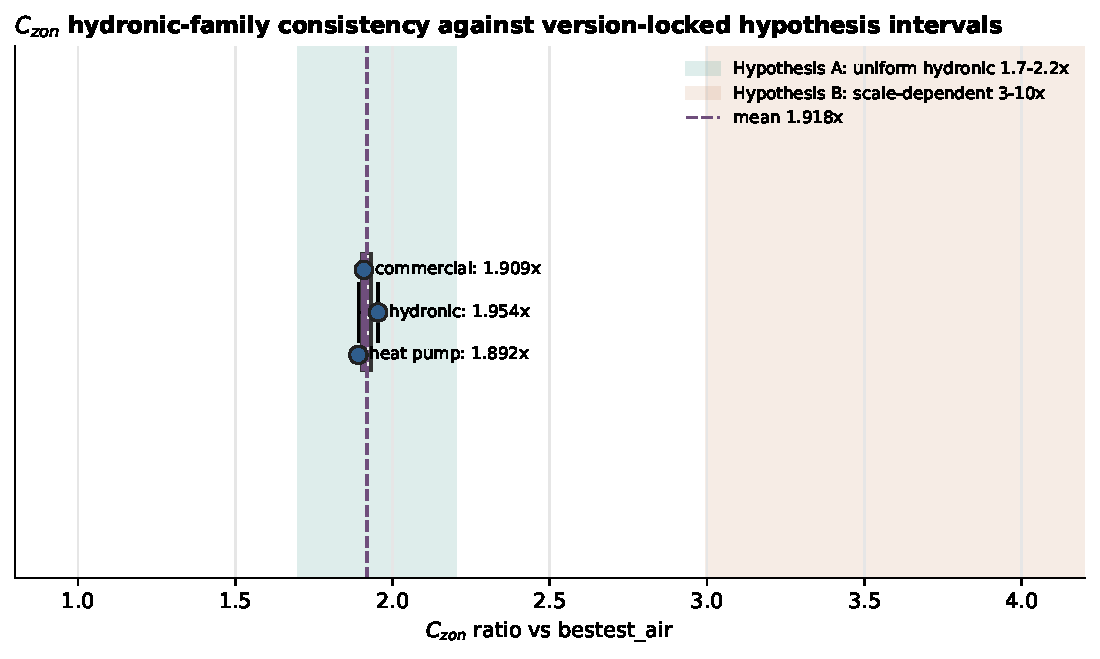
\includegraphics[width=0.82\linewidth]{block3_q1_polish_czon_hypothesis_box.pdf}
  \caption{$C_{\mathrm{zon}}$ re-identification as a horizontal box/point
  diagnostic over pre-registered hypothesis intervals. The observations cluster
  inside Hypothesis A (uniform hydronic family, $1.7$--$2.2\times$) and away
  from Hypothesis B (scale-dependent, $3$--$10\times$).}
  \label{fig:czon_consistency}
\end{figure}

\begin{figure}[t]
  \centering
  
\includegraphics[width=0.82\linewidth]{final_eng_fig12_czon_hypothesis_interval.pdf}
  \caption{$C_{\mathrm{zon}}$ hypothesis interval plot. The observed commercial ratio falls inside the uniform hydronic-family hypothesis interval and outside the scale-dependent interval.}
  \label{fig:czon_hypothesis}
\end{figure}

\begin{figure}[t]
  \centering
  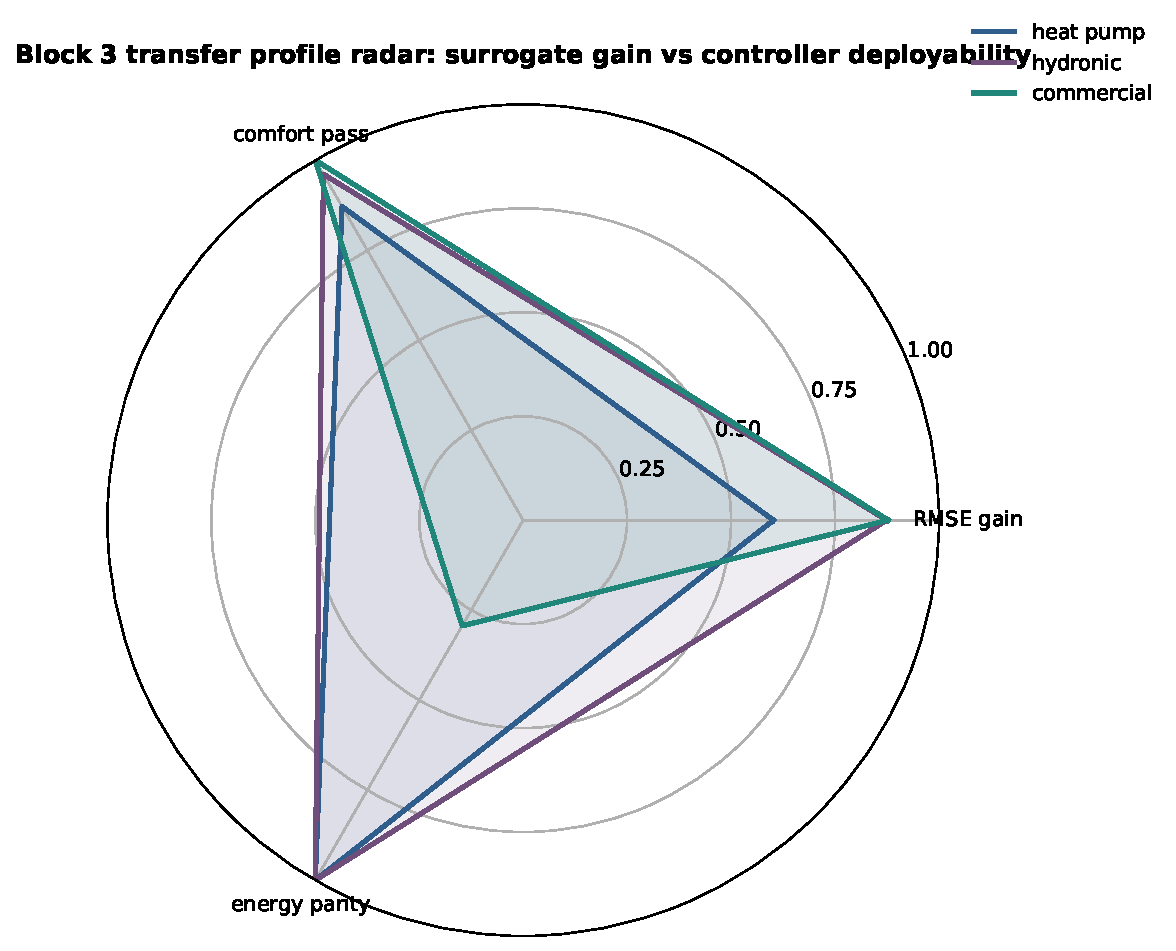
\includegraphics[width=0.82\linewidth]{block3_q1_polish_transfer_radar.pdf}
  \caption{Transfer-profile radar chart. Each target testcase is summarized by
  surrogate RMSE gain, threshold-normalized comfort pass score, and energy
  parity. The figure visualizes the component-level result: surrogate
  transferability is strong, while controller deployability is
  testcase-regime-dependent.}
  \label{fig:transfer_radar}
\end{figure}

\section{Hypothesis closure}

Table~\ref{tab:hypothesis} closes the pre-registered hypotheses. The most important methodological point is that Block 3 does not collapse the evidence into a single pass/fail label. Surrogate transfer and controller transfer diverge.

\begin{table}[t]
\centering
\caption{Pre-registered hypothesis closure.}
\label{tab:hypothesis}
\small
\begin{tabular}{>{\raggedright\arraybackslash}p{26mm}>{\raggedright\arraybackslash}p{40mm}>{\raggedright\arraybackslash}p{28mm}>{\raggedright\arraybackslash}p{54mm}}
\toprule
Hypothesis & Claim & Verdict & Evidence \\
\midrule
H1 strong & Frozen recipe transfers in mode=none & Falsified & Residential hydronic testcases fail the $1.25\times$ PI threshold; commercial is threshold-pass only with $+35.33\%$ energy. \\
H2 medium & Partial Stage C is enough for controller transfer & Falsified structurally & Partial recalibrates the surrogate only; controller is frozen, so live KPI cannot improve without excluded fine-tuning. \\
H3 weak, surrogate side & Full Stage A/B/C gives usable target surrogate & Supported on N=3 & RMSE gains: $60.2\%$, $87.4\%$, $87.8\%$; $C_{\mathrm{zon}}$ consistently re-identified. \\
H3 weak, controller side & Frozen controller transfers with valid adapters & Falsified / regime-dependent & Residential cases fail comfort; commercial passes threshold but overuses energy. \\
Hierarchy consistency & Regime ordering does not contradict definitions & Supported & Controller KPI is invariant under surrogate-only recalibration; surrogate fidelity improves with full recalibration. \\
\bottomrule
\end{tabular}
\end{table}

\begin{figure}[t]
  \centering
  
\includegraphics[width=0.88\linewidth]{final17_fig17_hypothesis_closure_matrix.pdf}
  \caption{Hypothesis closure matrix. Block 3 supports surrogate-side transferability but falsifies deployment-ready frozen-controller transfer.}
  \label{fig:hypothesis_closure}
\end{figure}

\section{Pre-registered stretch predictions versus outcomes}

The stretch testcase was not only a third datapoint; it was a falsification probe with numerical a-priori predictions. The observed outcomes are mixed in the desired scientific sense:
\begin{itemize}
  \item Mode=none controller verdict: expected FAIL with probability 0.80; observed threshold PASS. Prediction falsified.
  \item Full surrogate RMSE gain: expected $50$--$90\%$ with probability 0.70; observed $87.81\%$. Prediction supported.
  \item Uniform hydronic $C_{\mathrm{zon}}$ hypothesis: expected $1.7$--$2.2\times$ with probability 0.35; observed $1.909\times$. Supported.
  \item Scale-dependent $C_{\mathrm{zon}}$ hypothesis: expected $3$--$10\times$ with probability 0.50; observed $1.909\times$. Falsified.
  \item Pipeline-failure hypothesis: expected possible non-convergence with probability 0.15; Stage A/B/C converged. Falsified.
\end{itemize}
This predicted-versus-observed mapping is central to the audit trail. It shows that the manifest contained genuinely competing expectations and that the evidence moved the interpretation toward lower-prior hypotheses rather than confirming only what was expected.

\section{Results III conclusion}

Block 3 establishes a component-level transferability boundary. The inverse-calibration component of the v3.5 surrogate transfers strongly to the hydronic-family target testcases: full Stage A/B/C improves RMSE by $60$--$88\%$ and re-identifies $C_{\mathrm{zon}}$ at a consistent $1.918\pm0.032\times$ the \texttt{bestest\_air} value. This is the positive physical result.

The frozen controller component does not transfer as a deployment-ready policy. On the two residential hydronic testcases, the frozen controller saves energy but fails the comfort/safety threshold. On the commercial hydronic stretch case, the controller passes the $m_s$ threshold but consumes $35.33\%$ more energy than PI. This is a threshold pass, not a deployment-ready pass. The transferability boundary therefore lies at the controller-adapter interface, not in the surrogate's ability to recalibrate target physics.

The practical implication for Block 4 is precise: target-specific controller fine-tuning on the fully recalibrated surrogate is the next falsifiable step. Block 3 shows that the target surrogate is accurate enough to be a candidate training environment; it also shows that freezing the source controller is insufficient for deployment-ready hydronic transfer.

\end{document}
